\section{Referencial Teórico}
\label{sec:refteorico}

Esta seção apresenta os conceitos necessários ao desenvolvimento do conversor
CC-CC de três portas controlado pela técnica FCS-MPC: a modelagem de
conversores multiporta, a representação do painel fotovoltaico, os
fundamentos do controle preditivo baseado em modelo com conjunto finito de
controle (FCS-MPC) e os observadores de estado empregados na redução da
instrumentação do sistema.

\subsection{Conversores CC-CC de Três Portas}
\label{subsec:conversor3portas}

Conversores de três portas integram fonte, armazenamento e carga em um único
estágio de potência, reduzindo o número de componentes em relação ao uso de
conversores independentes \citep{zhang2025adaptive}. Na topologia VR-BESS
adotada neste trabalho (Fig.~\ref{fig:topologia}), duas chaves
semicondutoras e um indutor compartilhado regulam o fluxo de potência entre
as portas de geração fotovoltaica, armazenamento (BESS) e carga, operando
como conversor \textit{Buck} durante o carregamento da bateria e como
\textit{Boost} durante a regulação da tensão de saída.

\begin{figure}[h]
\centering
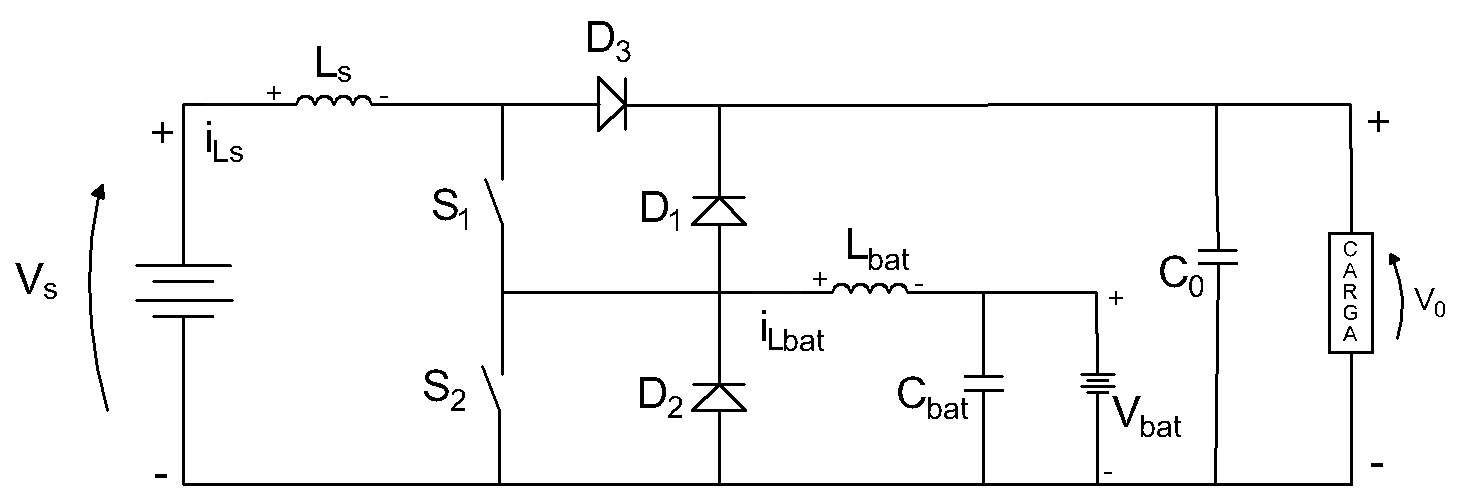
\includegraphics[width=\linewidth]{Figuras/topologia_3portas.png}
\caption{Representação conceitual da topologia de duas chaves do conversor
de três portas (FV--BESS--Carga).}
\label{fig:topologia}
\end{figure}

O modelo de valores médios de cada porta $x$ é obtido a partir do balanço de
carga no respectivo capacitor, podendo ser escrito de forma geral como

\begin{equation}
\dot V_x = \frac{1}{C_x}I_x - \frac{1}{C_x R_x}V_x,
\label{eq:portmodel}
\end{equation}

em que $I_x$ é a corrente injetada na porta, $C_x$ a capacitância
equivalente e $R_x$ a resistência de carga vista por essa porta
\citep{zhang2025adaptive}. A Eq.~\eqref{eq:portmodel}, aplicada a cada porta
do conversor, fundamenta a representação em espaço de estados sobre a qual o
controlador FCS-MPC atua.

\subsection{Modelagem do Painel Fotovoltaico}
\label{subsec:modelopv}

A porta de entrada do conversor é alimentada por um painel FV representado
pelo circuito equivalente de diodo único, cuja corrente de saída é função da
tensão nos terminais:

\begin{equation}
I_y = I_{SC}\left[1 - K_1\!\left(e^{V_y/(K_2 V_{OC})} - 1\right)\right],
\label{eq:pvmodel}
\end{equation}

em que $K_1$ e $K_2$ são obtidos a partir dos parâmetros de catálogo
($I_{SC}$, $I_{MP}$, $V_{OC}$, $V_{MP}$) nas condições padrão de teste
\citep{ayaz2014improved}. Esses parâmetros são corrigidos em função da
irradiância $G$ e da temperatura de célula $T_C$, sendo esta última estimada
a partir da temperatura ambiente, da irradiância e da velocidade do vento. O
modelo, validado experimentalmente para módulos monocristalinos,
policristalinos e de filme fino, apresentou desvios de energia entre $3,25\%$
e $13,93\%$ em relação aos dados medidos \citep{ayaz2014improved}, sendo
adotado neste trabalho para representar a fonte conectada à porta FV do
conversor.

\subsection{Controle Preditivo Baseado em Modelo com Conjunto Finito de Controle (FCS-MPC)}
\label{subsec:fcsmpc}

O FCS-MPC explora o número finito de estados de comutação de um conversor
para, a cada período de amostragem: (i) predizer o valor futuro das
variáveis de estado $x^P(k+1)$ para cada estado de comutação $S_n$
disponível; (ii) avaliar uma função de custo que pondera o erro entre
$x^{P}$ e a referência $x^{*}$; e (iii) aplicar o estado $S_{opt}$ que
minimiza essa função, repetindo o processo no instante seguinte
\citep{ferreira2018finite, wang2023fcsmpc} (Fig.~\ref{fig:fcsmpc}).

\begin{figure}[h]
\centering
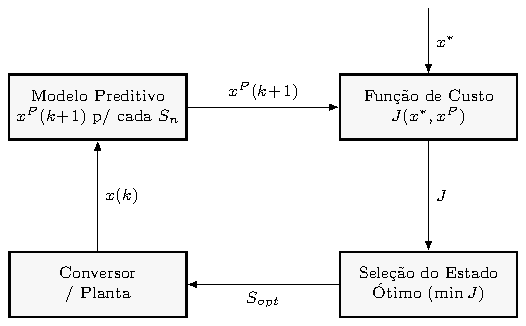
\includegraphics[width=\linewidth]{Figuras/fcsmpc_diagrama.pdf}
\caption{Estrutura genérica do controle FCS-MPC.}
\label{fig:fcsmpc}
\end{figure}

Para conversores com múltiplas variáveis controladas, a função de custo pode
ser definida de forma multivariável, ponderando o erro de cada variável por
um ganho independente, como em

\begin{equation}
J = K_1\left|x_1^{*} - x_1^{P}\right| + K_2\left|x_2^{*} - x_2^{P}\right|,
\label{eq:costfunction}
\end{equation}

em que $K_1$ e $K_2$ definem a prioridade relativa entre os objetivos de
controle \citep{ferreira2018finite}. O principal fator limitante do FCS-MPC é
o crescimento do esforço computacional com o número de estados de comutação
e com o horizonte de predição $N$; em conversores multinível, esse custo
pode ser reduzido por meio de estruturas híbridas que combinam redes
neurais com o próprio FCS-MPC, alcançando reduções de até $58,8\%$ no esforço
computacional \citep{wang2023fcsmpc}. Conversores com poucas chaves, como o
VR-BESS aqui adotado, possuem um conjunto de estados naturalmente reduzido,
o que favorece a aplicação direta do FCS-MPC sem a necessidade dessas
estruturas auxiliares.

\subsection{Observadores de Estado e Controle por Rejeição Ativa de Distúrbios}
\label{subsec:observadores}

Conversores multiporta apresentam acoplamento entre portas e incertezas
paramétricas que limitam o desempenho de controladores de ganho fixo
\citep{zhang2025adaptive}. O controle por rejeição ativa de distúrbios (ADRC)
trata essas incertezas, em conjunto com dinâmicas não modeladas, como um
\textit{distúrbio total}, estimado em tempo real por um observador de
estados estendido (ESO) e compensado na lei de controle.

Para melhorar simultaneamente a imunidade a ruído em regime permanente e o
rastreamento durante transitórios, pode-se empregar um observador
adaptativo (AESO) que alterna entre um observador linear tradicional
(TLESO) e um observador baseado em malha de captura de fase (PLLO),
conforme a Fig.~\ref{fig:aeso}. A comutação é definida por um limiar de erro

\begin{equation}
\mu = \Delta V + \delta,
\label{eq:threshold}
\end{equation}

combinado a temporizadores de confirmação ($t_{1d}$, $t_{2d}$) que evitam
comutações espúrias \citep{zhang2025adaptive}.

\begin{figure}[h]
\centering
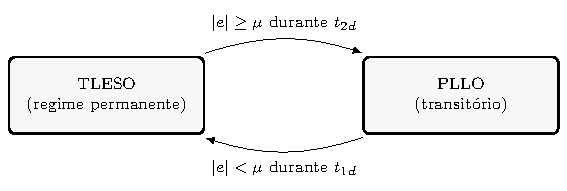
\includegraphics[width=\linewidth]{Figuras/aeso_diagrama.pdf}
\caption{Lógica de comutação entre os observadores TLESO e PLLO.}
\label{fig:aeso}
\end{figure}

Embora o presente trabalho adote o FCS-MPC como estratégia principal de
controle, o uso de observadores de estado é relevante para a etapa de
simulação prevista neste TCC, na qual se pretende avaliar sua aplicação como
alternativa para reduzir o número de sensores físicos necessários à
implementação do controle preditivo no conversor VR-BESS.
